\documentclass{standalone}
\usepackage{tikz}
\usetikzlibrary{calc} % 坐标计算库
\usetikzlibrary{patterns} % 阴影填充库
\usepackage{pgfplots} % 绘图库
\usepgfplotslibrary{fillbetween} % 区域阴影
\pgfplotsset{compat=1.18} % 设置 pgfplots 版本
\usetikzlibrary{patterns.meta} % 图案库

% 常量声明
\newcommand{\xmin}{0}
\newcommand{\xmax}{7}
\newcommand{\ymin}{-13}
\newcommand{\ymax}{23}

\begin{document}

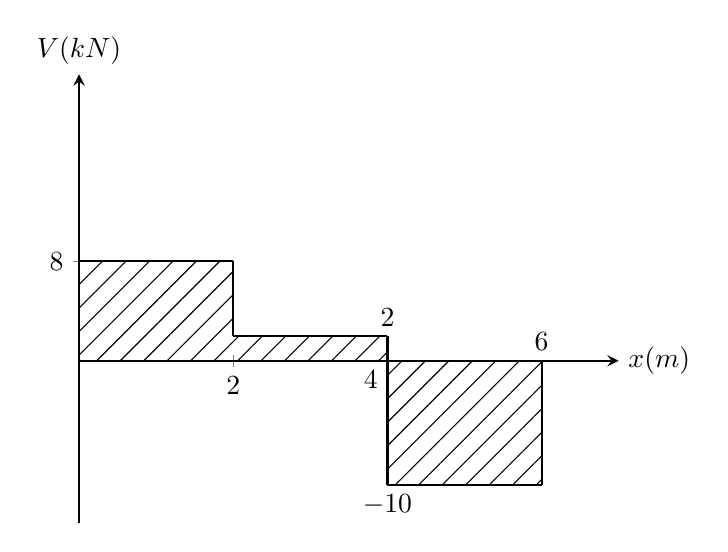
\begin{tikzpicture}
    % Shear Diagram
    \begin{axis}[
            axis lines=middle, % 学校式坐标轴
            axis line style={thick},
            xlabel={$x(m)$},
            xlabel style={right},
            ylabel={$V(kN)$},
            ylabel style={above},
            xtick={2},
            % xticklabel style={anchor=south, yshift=4pt},
            ytick={8},
            xmin=\xmin, xmax=\xmax,
            ymin=\ymin, ymax=\ymax,
            domain=0:3,
        ]
        % 定义函数和x轴
        \addplot[name path=A, domain=0:2, thick] {8};
        \addplot[name path=B, domain=2:4, thick] {2};
        \addplot[name path=C, domain=4:6, thick] {-10};
        \addplot[name path=AA, domain=0:2] {0};
        \addplot[name path=BB, domain=2:4] {0};
        \addplot[name path=CC, domain=4:6] {0};
        % 填充两者之间的区域
        \addplot[
            pattern={Lines[angle=45, distance=6pt]},
        ] fill between [of=A and AA];
        \addplot[
            pattern={Lines[angle=45, distance=6pt]},
        ] fill between [of=B and BB];
        \addplot[
            pattern={Lines[angle=45, distance=6pt]},
        ] fill between [of=C and CC];
        % 添加标识线或点
        \node at (axis cs:4,0) [below left] {$4$};
        \node at (axis cs:6,0) [above] {$6$};
        \node at (axis cs:4,2) [above] {$2$};
        \node at (axis cs:4,-10) [below] {$-10$};
        \draw[thick] (axis cs:2,2) -- (axis cs:2,8);
        \draw[thick] (axis cs:4,2) -- (axis cs:4,-10);
        \draw[thick] (axis cs:6,0) -- (axis cs:6,-10);
    \end{axis}

\end{tikzpicture}

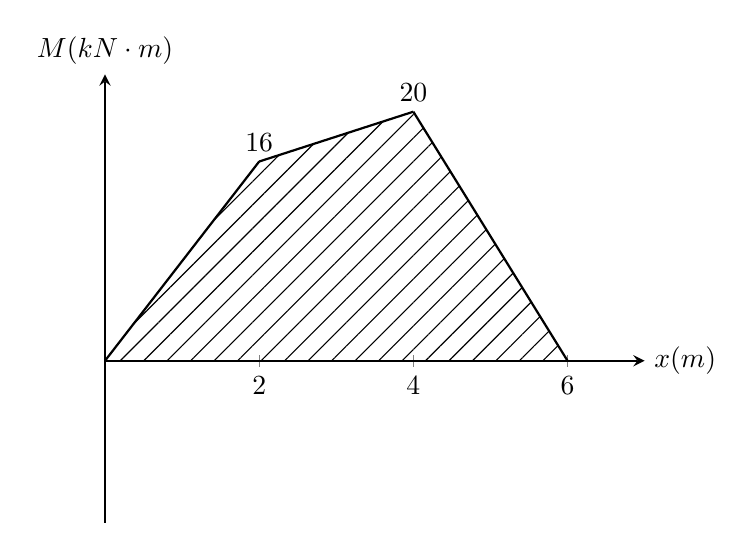
\begin{tikzpicture}
    % Moment Diagram
    \begin{axis}[
            axis lines=middle, % 学校式坐标轴
            axis line style={thick},
            xlabel={$x(m)$},
            xlabel style={right},
            ylabel={$M(kN \cdot m)$},
            ylabel style={above},
            xtick={2,4,6},
            % xticklabel style={anchor=south, yshift=4pt},
            ytick=\empty,
            xmin=\xmin, xmax=\xmax,
            ymin=\ymin, ymax=\ymax,
            domain=0:6,
        ]
        % 定义函数和x轴
        \addplot[name path=A, domain=0:2, thick] {8*x};
        \addplot[name path=B, domain=2:4, thick] {8*x-6*(x-2)};
        \addplot[name path=C, domain=4:6, thick] {8*x-6*(x-2)-12*(x-4)};
        \addplot[name path=AA, domain=0:2] {0};
        \addplot[name path=BB, domain=2:4] {0};
        \addplot[name path=CC, domain=4:6] {0};
        % 填充两者之间的区域
        \addplot[
            pattern={Lines[angle=45, distance=6pt]},
        ] fill between [of=A and AA];
        \addplot[
            pattern={Lines[angle=45, distance=6pt]},
        ] fill between [of=B and BB];
        \addplot[
            pattern={Lines[angle=45, distance=6pt]},
        ] fill between [of=C and CC];
        % 添加标识线或点
        \node at (axis cs:2,16) [above] {$16$};
        \node at (axis cs:4,20) [above] {$20$};
    \end{axis}

\end{tikzpicture}

\end{document}